\documentclass{beamer}
\usepackage{pgfpages}
%\setbeameroption{show notes on second screen=left} %enable for notes
\usepackage{graphicx}
\usepackage{xcolor}
\usepackage{listings}
%\usepackage{transparent}
\usepackage{hyperref}
\lstset{language=python,frame=single}
\usepackage{verbatim}
%\usepackage{apacite}
\usepackage[longnamesfirst]{natbib}
\usepackage{subcaption}
\usepackage{amsmath}
\usepackage{relsize}
\usepackage{appendixnumberbeamer}
\usepackage{xparse}
\usepackage{multimedia}
\usepackage{xcolor}
\usepackage[normalem]{ulem}
\usepackage{tikz}
\usetikzlibrary{matrix,backgrounds}
\usetikzlibrary{positioning}
\usetikzlibrary{shapes,arrows}
\usetikzlibrary{positioning}

\tikzset{onslide/.code args={<#1>#2}{%
  \only<#1>{\pgfkeysalso{#2}} 
}}

\tikzstyle{block} = [rectangle, draw, fill=red!20!blue!10, 
    text width=5em, text centered, rounded corners, minimum height=4em]
\tikzstyle{netnode} = [circle, draw, very thick, inner sep=0pt, minimum size=0.5cm] 
\tikzstyle{relunode} = [rectangle, draw, very thick, inner sep=0pt, minimum size=0.5cm] 
    
\tikzstyle{line} = [draw, line width=1.5pt, -latex']

\pgfdeclarelayer{background}
\pgfsetlayers{background,main}

\pgfdeclarelayer{myback}
\pgfsetlayers{myback,background,main}

\usetheme[numbering=fraction]{metropolis}
\newcommand{\semitransp}[2][35]{\color{fg!#1}#2}

\newcommand\blfootnote[1]{%
  \begingroup
  \renewcommand\thefootnote{}\footnote{#1}%
  \addtocounter{footnote}{-1}%
  \endgroup
}
\renewcommand*\footnoterule{}
%%\AtBeginSection[]
%%{
%%  \begin{frame}
%%    \frametitle{Table of Contents}
%%    \tableofcontents[currentsection]
%%  \end{frame}
%%}

\begin{document}

\title{Multi-task learning, generalization, and abstraction}
\author{Andrew Lampinen\\
PhD Candidate, Psychology\\
Stanford University}
\date{}
\frame{\titlepage}

\begin{frame}[standout]
Connectionist modeling has too often focused on single tasks.\par
\end{frame}

\begin{frame}{Prior work on multiple tasks in neural networks}
\begin{figure}
\centering
\only<2> {
\includegraphics[height=0.75\textheight]{figures/rm_sem_task.png}
} \only<3> {
\includegraphics[height=0.75\textheight]{figures/rm_sem_reps.png}
} \only<4> {
\includegraphics[height=0.75\textheight]{figures/dag_transf.png}
}
\end{figure}
\blfootnote{
    \only<2-3>{\citep{Hinton1986, Rogers2008}}
    \only<4->{\citep{Dienes1999}}
}
\end{frame}

\begin{frame}[fragile]{Multi-task learning can substantially improve generalization}
\uncover<2->{
\begin{figure}
\centering
\begin{tikzpicture}[remember picture, overlay, every node/.style={inner sep=0,outer sep=0}]
\node [anchor=center, draw, fill=white, minimum width=2cm, minimum height= 1 cm] at (current page.center) (brain) {\Large RNN};
\only<-4>{
\node [anchor=center, below left = 1cm and 0.25cm of brain] (input1) {``Ceci n'est pas une pipe.''};
\node [anchor=center, above left = 1cm and 0.25cm of brain] (output1) {``This is not a pipe.''};
}

\only<-4>{
\node<3-4> [anchor=center, below right = 0.45cm and 0.25cm of brain] (input2) {\includegraphics[width=0.25\textwidth]{figures/un_pipe.jpg}};
\node<3-4> [anchor=center, above right = 1cm and 0.25cm of brain] (output2) {``This is a pipe.''};
}

\only<5->{
\node [anchor=center, below left = 1.25cm and 1cm of brain] (mi1) {French};
\node [anchor=center, above left = 1.25cm and 1cm of brain] (mo1) {Chinese};
\node [anchor=center, below left = 2cm and -0.25cm of brain] (mi2) {Swahili};
\node [anchor=center, above left = 2cm and -0.25cm of brain] (mo2) {German};

\node [anchor=center, below right = 1.25cm and 1cm of brain] (mi4) {English};
\node [anchor=center, above right = 1.25cm and 1cm of brain] (mo4) {Italian};
\node [anchor=center, below right = 2cm and -0.25cm of brain] (mi3) {Spanish};
\node [anchor=center, above right = 2cm and -0.25cm of brain] (mo3) {Korean};
}

\begin{pgfonlayer}{background}
\only<-4>{
\path [line] (input1.east) to [out=45, in=-45] (output1.east);
\path<3-4> [line] (input2.west) to [out=135, in=-135] (output2.west);
}
\only<5->{
\path [line] (mi1.east) to [out=10, in=-10] (mo1.east);
\path [line] (mi2.north east) to [out=70, in=-70] (mo2.south east);
\path [line] (mi4.west) to [out=170, in=-170] (mo4.west);
\path [line] (mi3.north west) to [out=110, in=-110] (mo3.south west);
}
\end{pgfonlayer}
\only<4>{
\path [line, line width=3 pt, red, dashed] ([xshift=0.44cm]input1.north) to node [anchor=center, text width=2.5cm, align=center, xshift=-1.5cm] {Better generalization!} (output1.south);
}
\only<6->{
\path [line, line width=3 pt, red, dashed] (mi4.west) to node [anchor=center, xshift=3cm] {No training needed!} (mo1.east);
}
\end{tikzpicture}
\end{figure}
\vspace{2em}
\blfootnote{\uncover<4->{
    \only<2-4>{\citep*{Luong2016}}
    \only<1,5->{\citep{Johnson2016a}}
}}
}
\end{frame}

\begin{frame}[standout]
Multi-task learning can substantially improve generalization in neural networks.\par
\end{frame}


\begin{frame}<2->{Multi-task learning in humans}
\begin{itemize}
\item Humans do many related tasks!
\item<3-> The idea that transfer is beneficial to humans isn't new.
\item<4-> However, previous transfer research mostly focused on subjects rapidly finding explicit analogies in toy domains, with limited success.
\item<5-> The neural network research suggests instead that transfer might be more useful over \textbf{slower timescales} in \textbf{more complex tasks}, and possibly \textbf{without explicit awareness}.
\end{itemize}
\vspace{2em}
\blfootnote{
    \only<1-4>{\citep{Gentner2003, Day2011}}
    \only<1,5->{\citep{Lampinen2017a, Bransford1999}}
}

\end{frame}

\begin{frame}{Humans face many related tasks}
\begin{figure}
\centering
\begin{subfigure}{0.4\textwidth}
\includegraphics[width=\textwidth]{figures/chess_cropped.jpg}
\end{subfigure}%
\begin{subfigure}{0.4\textwidth}
\includegraphics[width=\textwidth]{figures/go2.jpg}
\end{subfigure}\\
\uncover<2>{
\begin{subfigure}{0.4\textwidth}
\includegraphics[width=\textwidth]{figures/math.jpg}
\end{subfigure}%
\begin{subfigure}{0.4\textwidth}
\includegraphics[width=\textwidth]{figures/piano.jpg}
\end{subfigure}%
}
\end{figure}
\uncover<2->{
\scriptsize
\citep{Lampinen2017a, Hansen2017}
}
\note{There are deep relationships among the tasks we do -- some are superficially obvious, like Go and Chess, and some are less so, like the mathematical structures underlying music or the fact that we use language to talk about all these domains.}
\end{frame}

\begin{frame}{Multi-task learning can also be beneficial on smaller scales}
\begin{figure}
\centering
\begin{subfigure}{0.3\textwidth}
\uncover<2->{
\includegraphics[width=\textwidth]{figures/hexagon_arrow.png}
}
\end{subfigure}~
\begin{subfigure}{0.65\textwidth}
\uncover<3->{
\includegraphics[width=\textwidth]{figures/fyp_1_modular_text.png}
}
\end{subfigure}
\end{figure}
\vspace{1.5em}
\begin{itemize}
\item<4-> Participants who saw hybrid of both performed better!
\item<5-> Importantly, the benefit of seeing both only emerged \textbf{slowly}, after subjects had worked with the materials for a while.
\end{itemize}
\vspace{1.5em}
{
\scriptsize
\citep{Lampinen2017b}
}
\end{frame}

\begin{frame}[standout]
Our models should reflect the fact that human intelligence is multi-purpose.\par
\end{frame}

\begin{frame}{Multi-task benefits (and costs)}
\begin{figure}
\centering
\only<2>{
\vspace{3em}
\includegraphics[width=\textwidth]{figures/analytic_paper_title.png}
}
\only<3>{
\vspace{3em}
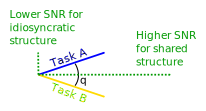
\includegraphics[width=0.8\textwidth]{figures/transfer_pros_cons.png}
\vspace{1.25em}
}
\only<4>{
\vspace{2em}
\begin{subfigure}{0.3\textwidth}
\includegraphics[width=\textwidth]{figures/fig_5a.png}
\end{subfigure}~
\begin{subfigure}{0.3\textwidth}
\includegraphics[width=\textwidth]{figures/transfer_by_alignment.png}
\end{subfigure}~
\begin{subfigure}{0.4\textwidth}
\includegraphics[width=\textwidth]{figures/fig_5c.png}
\end{subfigure}
%%\includegraphics[width=0.5\textwidth]{figures/transfer_by_alignment.png}
}
\end{figure}
\end{frame}


\begin{frame}[standout]
When the target task is noisy or auxiliary tasks are well aligned, transfer is very beneficial.
\end{frame}

\begin{frame}[fragile]{Limitations of deep learning, or of tasks?}
Neural networks are often criticized for needing more data than humans to learn a task. \uncover<2->{But:}
\begin{itemize}
\item<2-> Not enough data $=$ small SNR.
\item<3-> Most tasks humans learn are related to other things we do. 
\end{itemize}
\uncover<4->{ So this is the domain where transfer can be most beneficial! (Noisy tasks with aligned auxiliary tasks.)}
%\begin{figure}
%\vspace{-2em}
%\centering
%\begin{tikzpicture}[remember picture, overlay, every node/.style={inner sep=0,outer sep=0}]
%\node [anchor=center, align=center,] at (-1, 0) (c0) {\includegraphics[width=7cm]{figures/critique0.png}};
%\node [anchor=center, align=center,] at (0, 0) (c1) {\includegraphics[width=7cm]{figures/critique1.png}};
%\node [anchor=center, align=center,] at (1, -2) (c2) {\includegraphics[width=7cm]{figures/critique2.png}};
%\end{tikzpicture}
%\end{figure}
%\vspace{2em}
\end{frame}

\begin{frame}[standout]
Data-hunger and failures to generalize may be due to ``poverty of the tasks'' -- we do many more tasks than our models.\par
\end{frame}

\begin{frame}{Abstraction \& transfer}
\begin{itemize}
\item ``Transfer'' usually considered between similar tasks.
\item <2->In math (and other domains) we often do tasks that are related by abstraction. 
\item <3->Work on grounding, e.g. in gesture \cite{Wakefield2018}.
\item <4->Do more basic tasks help set up representations for more abstract ones?
\end{itemize}
\begin{figure}
\centering
\only<-4>{\vspace{0.5\textheight}}
\only<5> {
\includegraphics[height=0.5\textheight]{figures/rm_sem_reps.png}
}
\only<6>{
\includegraphics[height=0.5\textheight]{figures/man_woman.jpg}
}
\only<7>{
\vspace{0.75em}
\begin{subfigure}{0.5\textwidth}
\includegraphics[width=\textwidth]{figures/group_14_1.png}
\end{subfigure}~
\begin{subfigure}{0.5\textwidth}
\includegraphics[width=\textwidth]{figures/group_14_2.png}
\end{subfigure}
}
\end{figure}
\end{frame}

\begin{frame}[standout]
Does the structure that emerges in our representations when learning basic tasks prepare us for abstraction?
\end{frame}


\begin{frame}[fragile]{Acknowledgements}
\vspace{1em}
\begin{figure}
\centering
\begin{tikzpicture}[remember picture, overlay]
\node at (-2, 1.5) {\includegraphics[width=2cm]{figures/people/jay.jpg}};
\node<2-> at (2, 1.5) {\includegraphics[width=2cm]{figures/people/surya.jpg}};

\node<3-> at (-4, -1.5) {\includegraphics[width=2cm]{figures/people/arianna.jpg}};
\node<3-> at (0, -1.5) {\includegraphics[width=2cm]{figures/people/katherine.jpg}};
\end{tikzpicture}
\end{figure}
\end{frame}

\begin{frame}[allowframebreaks]
\bibliographystyle{plainnat}
{\bibliography{transfer}}
\end{frame}

\end{document}


